\documentclass[10pt,a4paper]{article}
\usepackage[margin=2.1cm]{geometry}
\usepackage{amsmath,amssymb,bm}
\usepackage{graphicx,booktabs,caption,subcaption}
\usepackage[hidelinks]{hyperref}
\usepackage{lmodern}          % scalable fonts (microtype expansion needs them)
\usepackage[T1]{fontenc}
\usepackage{microtype}
\usepackage{xcolor}
\usepackage{placeins}
\captionsetup{font=small,labelfont=bf}
\newcommand{\NL}{63}
\newcommand{\Mtrain}{29\,312}
\newcommand{\Mtest}{7\,401}
\newcommand{\Mnovel}{7401}
\newcommand{\Mcopies}{0}
\newcommand{\PctCopies}{0}
\newcommand{\ThetaTrain}{0.312}
\newcommand{\MeffTrain}{3590}
\newcommand{\ThetaTest}{0.303}
\newcommand{\MeffTest}{1280}
\newcommand{\MeffNovel}{1280}
\newcommand{\NfOne}{1\,323}
\newcommand{\NCij}{861\,273}
\newcommand{\Hbest}{128}
\newcommand{\dbest}{10}
\newcommand{\lambest}{10^{-3}}
\newcommand{\Nparams}{217\,728}
\newcommand{\BestEpoch}{668}
\newcommand{\ValNLPL}{82.18}
\newcommand{\NLPLtrain}{71.10}
\newcommand{\NLPLtest}{78.72}
\newcommand{\NLPLnovel}{78.72}
\newcommand{\NLPLgap}{7.6}
\newcommand{\NLPLgapPct}{11}
\newcommand{\NLPLtestSite}{1.25}
\newcommand{\PPVL}{0.83}
\newcommand{\PPVLhalf}{1.00}
\newcommand{\PPVbase}{0.21}
\newcommand{\PCone}{11.3}
\newcommand{\PCtwo}{4.3}
\newcommand{\Etest}{-131.7}
\newcommand{\Etrain}{-134.3}
\newcommand{\Erandom}{-0.0}
\newcommand{\HamTestTest}{0.60}
\newcommand{\HamTestNN}{0.12}
\newcommand{\HamNovelTrain}{0.18}
\newcommand{\HamTestTrain}{0.18}
\newcommand{\rCtrain}{0.944}
\newcommand{\rCprof}{-0.005}
\newcommand{\sCtrain}{0.88}
\newcommand{\Crel}{0.94}
\newcommand{\sCdisTrain}{0.94}
\newcommand{\sCdisOne}{0.83}
\newcommand{\sCdisStar}{0.91}
\newcommand{\rCnovelFull}{1.000}
\newcommand{\BetaStar}{1.05}
\newcommand{\TauOne}{6.5}
\newcommand{\TauPOne}{3.8}
\newcommand{\BurnOne}{500}
\newcommand{\NgenOne}{10\,000}
\newcommand{\NcolOne}{0}
\newcommand{\PctColOne}{0.0}
\newcommand{\StudyColNatOne}{0.0}
\newcommand{\StudyColRndOne}{0.0}
\newcommand{\HamEndOne}{0.66}
\newcommand{\SweepsNinetyOne}{11}
\newcommand{\EendNatOne}{-126.6}
\newcommand{\EendRndOne}{-126.6}
\newcommand{\EgenOne}{-125.9}
\newcommand{\rFOne}{0.990}
\newcommand{\rCOne}{0.871}
\newcommand{\sCOne}{0.78}
\newcommand{\rCnovelOne}{0.871}
\newcommand{\HamGGOne}{0.68}
\newcommand{\HamGTOne}{0.44}
\newcommand{\HamGTrOne}{0.42}
\newcommand{\HamGTrMinOne}{0.32}
\newcommand{\UniqOne}{100.0}
\newcommand{\StudySweeps}{2000}
\newcommand{\WPCaOne}{0.26}
\newcommand{\WPCbOne}{0.34}
\newcommand{\WEOne}{5.9}
\newcommand{\TauStar}{5.6}
\newcommand{\TauPStar}{3.4}
\newcommand{\BurnStar}{500}
\newcommand{\NgenStar}{10\,000}
\newcommand{\NcolStar}{0}
\newcommand{\PctColStar}{0.0}
\newcommand{\StudyColNatStar}{0.0}
\newcommand{\StudyColRndStar}{0.0}
\newcommand{\HamEndStar}{0.64}
\newcommand{\SweepsNinetyStar}{17}
\newcommand{\EendNatStar}{-134.6}
\newcommand{\EendRndStar}{-134.6}
\newcommand{\EgenStar}{-133.8}
\newcommand{\rFStar}{0.992}
\newcommand{\rCStar}{0.859}
\newcommand{\sCStar}{0.85}
\newcommand{\rCnovelStar}{0.859}
\newcommand{\HamGGStar}{0.65}
\newcommand{\HamGTStar}{0.41}
\newcommand{\HamGTrStar}{0.39}
\newcommand{\HamGTrMinStar}{0.29}
\newcommand{\UniqStar}{100.0}
\newcommand{\WPCaStar}{0.30}
\newcommand{\WPCbStar}{0.31}
\newcommand{\WEStar}{2.1}
\newcommand{\WPCaTrain}{1.23}
\newcommand{\WPCbTrain}{0.29}
\newcommand{\WPCaProf}{1.05}
\newcommand{\WPCbProf}{0.66}
\newcommand{\WEtrain}{2.7}
\newcommand{\WEprof}{39.5}
\newcommand{\Eunw}{-146.2}
\newcommand{\ClTest}{14.1}
\newcommand{\ClTrain}{12.9}
\newcommand{\ClOne}{5.1}
\newcommand{\ClStar}{3.2}
\newcommand{\Kclust}{3}
\newcommand{\NcovClust}{2}
\newcommand{\CovWeight}{85.9}
\newcommand{\NtestCov}{6\,761}
\newcommand{\MeffTestCov}{1102}
\newcommand{\rCtrainCov}{0.941}
\newcommand{\rFcovOne}{0.991}
\newcommand{\rCcovOne}{0.918}
\newcommand{\sCcovOne}{0.82}
\newcommand{\rCcovTopOne}{0.961}
\newcommand{\rFcovStar}{0.996}
\newcommand{\rCcovStar}{0.918}
\newcommand{\sCcovStar}{0.91}
\newcommand{\rCcovTopStar}{0.961}
\newcommand{\NsuperSet}{36\,713}
\newcommand{\OrigCopies}{78.8}
\newcommand{\OrigNN}{0.044}
\newcommand{\SplitThresh}{0.2}
\newcommand{\SplitIdent}{80}
\newcommand{\NclustTot}{10\,942}
\newcommand{\NsingleClust}{6\,767}
\newcommand{\NtrainClean}{29\,312}
\newcommand{\NtestClean}{7\,401}
\newcommand{\NdropClean}{0}
\newcommand{\CleanNN}{0.179}
\newcommand{\CleanNNmin}{0.016}
\newcommand{\CleanNNminSub}{1}
\newcommand{\CleanNNmed}{0.175}
\newcommand{\CleanNNqfive}{0.032}
\newcommand{\CleanPctNear}{61}
\newcommand{\CleanDropRule}{exact}
\newcommand{\CmpMtrain}{14\,502}
\newcommand{\CmpMtest}{3\,739}
\newcommand{\CmpPctCopies}{79}
\newcommand{\CmpValNLPL}{85.61}
\newcommand{\CmpNLPLtest}{75.70}
\newcommand{\CmpNLPLnovel}{77.13}
\newcommand{\CmprFOne}{0.990}
\newcommand{\CmprCOne}{0.865}
\newcommand{\CmprCtrain}{0.960}
\newcommand{\CmpHamGTrOne}{0.42}
\newcommand{\CmpPPVLhalf}{0.97}
\newcommand{\CmprCcovOne}{0.921}
\newcommand{\MissCl}{C0}
\newcommand{\EmissTest}{-119.5}
\newcommand{\EmissTrain}{-122.6}
\newcommand{\EcovTest}{-134.0/-133.5}
\newcommand{\EcovTrain}{-134.5/-137.2}
\newcommand{\EgapMiss}{14}
\newcommand{\PLLmissTrain}{-71.8}
\newcommand{\PLLcovTrain}{-71.1/-71.0}
\newcommand{\dFmiss}{+1.01}
\newcommand{\dFmissFac}{0.36}

\newcommand{\ThermoEgap}{22.5}
\newcommand{\ThermoFgap}{2.8}
\newcommand{\ThermoSgap}{19.7}
\newcommand{\ThermoTable}{$\langle E\rangle_k-\langle E\rangle_{C1}=(22.5,\,0.0,\,9.3)$, $F_k-F_{C1}=(2.8,\,0.0,\,2.2)$ and therefore $S_k-S_{C1}=(19.7,\,0.0,\,7.1)$ for $k=$ C0, C1, C2}
\newcommand{\ShareBase}{5/86/9}
\newcommand{\dFzeroBase}{1.04}
\newcommand{\rfBase}{0.930}
\newcommand{\rCBase}{0.744}
\newcommand{\sCBase}{0.28}
\newcommand{\NLPLtestBase}{78.57}
\newcommand{\JfrobBase}{88.3}
\newcommand{\ShareMtwo}{5/83/12}
\newcommand{\dFzeroMtwo}{1.12}
\newcommand{\rfMtwo}{0.938}
\newcommand{\rCMtwo}{0.791}
\newcommand{\sCMtwo}{0.34}
\newcommand{\NLPLtestMtwo}{78.49}
\newcommand{\JfrobMtwo}{85.3}
\newcommand{\ShareNat}{14/39/47}
\newcommand{\FieldAbs}{0.95}
\newcommand{\ValBase}{81.97}
\newcommand{\EpBase}{962}
\newcommand{\ValMtwo}{82.03}
\newcommand{\EpMtwo}{962}
\newcommand{\ValCthree}{81.06}
\newcommand{\EpCthree}{791}
\newcommand{\ValCthreeQ}{80.02}
\newcommand{\EpCthreeQ}{1999}
\newcommand{\ValCthreeOne}{81.54}
\newcommand{\EpCthreeOne}{791}
\newcommand{\ValClean}{82.18}
\newcommand{\EpClean}{668}
\newcommand{\ValRepro}{82.18}
\newcommand{\EpRepro}{668}
\newcommand{\ShareClean}{5/36/59}
\newcommand{\ShareBasep}{5/86/9}
\newcommand{\NatEA}{-120.1}
\newcommand{\NatNA}{640}
\newcommand{\CeilA}{0.659}
\newcommand{\NatEB}{-135.2}
\newcommand{\NatNB}{4873}
\newcommand{\CeilB}{0.625}
\newcommand{\NatEC}{-133.3}
\newcommand{\NatNC}{1888}
\newcommand{\CeilC}{0.750}
\newcommand{\ConeALzerodist}{3.89}
\newcommand{\ConeALzeroover}{-3.47}
\newcommand{\ConeALzerorC}{0.154}
\newcommand{\ConeALzerorf}{0.683}
\newcommand{\ConeALzerohpd}{98}
\newcommand{\ConeALzeroE}{-126.3}
\newcommand{\ConeALzerodiv}{0.62}
\newcommand{\ConeALzerohit}{5}
\newcommand{\ConeALzerodtr}{0.39}
\newcommand{\ConeALQdist}{3.28}
\newcommand{\ConeALQover}{-2.96}
\newcommand{\ConeALQrC}{0.249}
\newcommand{\ConeALQrf}{0.761}
\newcommand{\ConeALQhpd}{98}
\newcommand{\ConeALQE}{-118.6}
\newcommand{\ConeALQdiv}{0.66}
\newcommand{\ConeALQhit}{18}
\newcommand{\ConeALQdtr}{0.43}
\newcommand{\ConeALonedist}{1.59}
\newcommand{\ConeALoneover}{-1.42}
\newcommand{\ConeALonerC}{0.436}
\newcommand{\ConeALonerf}{0.963}
\newcommand{\ConeALonehpd}{96}
\newcommand{\ConeALoneE}{-105.4}
\newcommand{\ConeALonediv}{0.70}
\newcommand{\ConeALonehit}{80}
\newcommand{\ConeALonedtr}{0.48}
\newcommand{\ConeALfourdist}{0.56}
\newcommand{\ConeALfourover}{-0.41}
\newcommand{\ConeALfourrC}{0.458}
\newcommand{\ConeALfourrf}{0.982}
\newcommand{\ConeALfourhpd}{96}
\newcommand{\ConeALfourE}{-106.3}
\newcommand{\ConeALfourdiv}{0.64}
\newcommand{\ConeALfourhit}{100}
\newcommand{\ConeALfourdtr}{0.46}
\newcommand{\ConeALonesixdist}{0.29}
\newcommand{\ConeALonesixover}{-0.13}
\newcommand{\ConeALonesixrC}{0.373}
\newcommand{\ConeALonesixrf}{0.969}
\newcommand{\ConeALonesixhpd}{96}
\newcommand{\ConeALonesixE}{-108.6}
\newcommand{\ConeALonesixdiv}{0.61}
\newcommand{\ConeALonesixhit}{100}
\newcommand{\ConeALonesixdtr}{0.44}
\newcommand{\ConeALsixfourdist}{0.15}
\newcommand{\ConeALsixfourover}{-0.04}
\newcommand{\ConeALsixfourrC}{0.307}
\newcommand{\ConeALsixfourrf}{0.964}
\newcommand{\ConeALsixfourhpd}{96}
\newcommand{\ConeALsixfourE}{-109.9}
\newcommand{\ConeALsixfourdiv}{0.60}
\newcommand{\ConeALsixfourhit}{100}
\newcommand{\ConeALsixfourdtr}{0.44}
\newcommand{\ConeBLzerodist}{1.51}
\newcommand{\ConeBLzeroover}{-1.34}
\newcommand{\ConeBLzerorC}{0.436}
\newcommand{\ConeBLzerorf}{0.992}
\newcommand{\ConeBLzerohpd}{99}
\newcommand{\ConeBLzeroE}{-126.6}
\newcommand{\ConeBLzerodiv}{0.62}
\newcommand{\ConeBLzerohit}{86}
\newcommand{\ConeBLzerodtr}{0.39}
\newcommand{\ConeBLQdist}{1.14}
\newcommand{\ConeBLQover}{-1.00}
\newcommand{\ConeBLQrC}{0.494}
\newcommand{\ConeBLQrf}{0.995}
\newcommand{\ConeBLQhpd}{99}
\newcommand{\ConeBLQE}{-129.0}
\newcommand{\ConeBLQdiv}{0.59}
\newcommand{\ConeBLQhit}{95}
\newcommand{\ConeBLQdtr}{0.38}
\newcommand{\ConeBLonedist}{0.86}
\newcommand{\ConeBLoneover}{-0.72}
\newcommand{\ConeBLonerC}{0.467}
\newcommand{\ConeBLonerf}{0.993}
\newcommand{\ConeBLonehpd}{99}
\newcommand{\ConeBLoneE}{-133.1}
\newcommand{\ConeBLonediv}{0.56}
\newcommand{\ConeBLonehit}{100}
\newcommand{\ConeBLonedtr}{0.36}
\newcommand{\ConeBLfourdist}{0.54}
\newcommand{\ConeBLfourover}{-0.40}
\newcommand{\ConeBLfourrC}{0.391}
\newcommand{\ConeBLfourrf}{0.986}
\newcommand{\ConeBLfourhpd}{99}
\newcommand{\ConeBLfourE}{-139.5}
\newcommand{\ConeBLfourdiv}{0.52}
\newcommand{\ConeBLfourhit}{100}
\newcommand{\ConeBLfourdtr}{0.33}
\newcommand{\ConeBLonesixdist}{0.29}
\newcommand{\ConeBLonesixover}{-0.15}
\newcommand{\ConeBLonesixrC}{0.304}
\newcommand{\ConeBLonesixrf}{0.978}
\newcommand{\ConeBLonesixhpd}{99}
\newcommand{\ConeBLonesixE}{-144.5}
\newcommand{\ConeBLonesixdiv}{0.48}
\newcommand{\ConeBLonesixhit}{100}
\newcommand{\ConeBLonesixdtr}{0.30}
\newcommand{\ConeBLsixfourdist}{0.16}
\newcommand{\ConeBLsixfourover}{-0.05}
\newcommand{\ConeBLsixfourrC}{0.262}
\newcommand{\ConeBLsixfourrf}{0.975}
\newcommand{\ConeBLsixfourhpd}{99}
\newcommand{\ConeBLsixfourE}{-146.9}
\newcommand{\ConeBLsixfourdiv}{0.47}
\newcommand{\ConeBLsixfourhit}{100}
\newcommand{\ConeBLsixfourdtr}{0.29}
\newcommand{\ConeCLzerodist}{3.28}
\newcommand{\ConeCLzeroover}{-3.06}
\newcommand{\ConeCLzerorC}{0.342}
\newcommand{\ConeCLzerorf}{0.728}
\newcommand{\ConeCLzerohpd}{98}
\newcommand{\ConeCLzeroE}{-126.5}
\newcommand{\ConeCLzerodiv}{0.62}
\newcommand{\ConeCLzerohit}{10}
\newcommand{\ConeCLzerodtr}{0.39}
\newcommand{\ConeCLQdist}{2.74}
\newcommand{\ConeCLQover}{-2.50}
\newcommand{\ConeCLQrC}{0.364}
\newcommand{\ConeCLQrf}{0.803}
\newcommand{\ConeCLQhpd}{98}
\newcommand{\ConeCLQE}{-122.4}
\newcommand{\ConeCLQdiv}{0.66}
\newcommand{\ConeCLQhit}{25}
\newcommand{\ConeCLQdtr}{0.42}
\newcommand{\ConeCLonedist}{1.05}
\newcommand{\ConeCLoneover}{-0.55}
\newcommand{\ConeCLonerC}{0.566}
\newcommand{\ConeCLonerf}{0.987}
\newcommand{\ConeCLonehpd}{98}
\newcommand{\ConeCLoneE}{-124.2}
\newcommand{\ConeCLonediv}{0.65}
\newcommand{\ConeCLonehit}{88}
\newcommand{\ConeCLonedtr}{0.44}
\newcommand{\ConeCLfourdist}{0.49}
\newcommand{\ConeCLfourover}{+0.00}
\newcommand{\ConeCLfourrC}{0.605}
\newcommand{\ConeCLfourrf}{0.993}
\newcommand{\ConeCLfourhpd}{99}
\newcommand{\ConeCLfourE}{-128.5}
\newcommand{\ConeCLfourdiv}{0.62}
\newcommand{\ConeCLfourhit}{100}
\newcommand{\ConeCLfourdtr}{0.43}
\newcommand{\ConeCLonesixdist}{0.29}
\newcommand{\ConeCLonesixover}{+0.03}
\newcommand{\ConeCLonesixrC}{0.539}
\newcommand{\ConeCLonesixrf}{0.992}
\newcommand{\ConeCLonesixhpd}{98}
\newcommand{\ConeCLonesixE}{-129.5}
\newcommand{\ConeCLonesixdiv}{0.61}
\newcommand{\ConeCLonesixhit}{100}
\newcommand{\ConeCLonesixdtr}{0.43}
\newcommand{\ConeCLsixfourdist}{0.15}
\newcommand{\ConeCLsixfourover}{+0.01}
\newcommand{\ConeCLsixfourrC}{0.509}
\newcommand{\ConeCLsixfourrf}{0.990}
\newcommand{\ConeCLsixfourhpd}{99}
\newcommand{\ConeCLsixfourE}{-129.2}
\newcommand{\ConeCLsixfourdiv}{0.61}
\newcommand{\ConeCLsixfourhit}{100}
\newcommand{\ConeCLsixfourdtr}{0.43}
\newcommand{\CthreeAsHKonedist}{0.42}
\newcommand{\CthreeAsHKoneover}{-0.14}
\newcommand{\CthreeAsHKonerC}{0.384}
\newcommand{\CthreeAsHKonerf}{0.968}
\newcommand{\CthreeAsHKonehpd}{100}
\newcommand{\CthreeAsHKoneE}{-118.4}
\newcommand{\CthreeAsHKonediv}{0.57}
\newcommand{\CthreeAsHKonehit}{100}
\newcommand{\CthreeAsHKonedtr}{0.42}
\newcommand{\CthreeAsHKtwodist}{0.91}
\newcommand{\CthreeAsHKtwoover}{+0.84}
\newcommand{\CthreeAsHKtworC}{0.219}
\newcommand{\CthreeAsHKtworf}{0.868}
\newcommand{\CthreeAsHKtwohpd}{100}
\newcommand{\CthreeAsHKtwoE}{-124.8}
\newcommand{\CthreeAsHKtwodiv}{0.45}
\newcommand{\CthreeAsHKtwohit}{100}
\newcommand{\CthreeAsHKtwodtr}{0.38}
\newcommand{\CthreeAsHKfourdist}{1.49}
\newcommand{\CthreeAsHKfourover}{+1.36}
\newcommand{\CthreeAsHKfourrC}{0.115}
\newcommand{\CthreeAsHKfourrf}{0.726}
\newcommand{\CthreeAsHKfourhpd}{100}
\newcommand{\CthreeAsHKfourE}{-120.1}
\newcommand{\CthreeAsHKfourdiv}{0.29}
\newcommand{\CthreeAsHKfourhit}{100}
\newcommand{\CthreeAsHKfourdtr}{0.39}
\newcommand{\CthreeAsHKeightdist}{1.65}
\newcommand{\CthreeAsHKeightover}{+1.47}
\newcommand{\CthreeAsHKeightrC}{0.081}
\newcommand{\CthreeAsHKeightrf}{0.635}
\newcommand{\CthreeAsHKeighthpd}{100}
\newcommand{\CthreeAsHKeightE}{-111.9}
\newcommand{\CthreeAsHKeightdiv}{0.16}
\newcommand{\CthreeAsHKeighthit}{100}
\newcommand{\CthreeAsHKeightdtr}{0.40}
\newcommand{\CthreeAsQKonedist}{0.32}
\newcommand{\CthreeAsQKoneover}{-0.04}
\newcommand{\CthreeAsQKonerC}{0.329}
\newcommand{\CthreeAsQKonerf}{0.965}
\newcommand{\CthreeAsQKonehpd}{100}
\newcommand{\CthreeAsQKoneE}{-119.2}
\newcommand{\CthreeAsQKonediv}{0.56}
\newcommand{\CthreeAsQKonehit}{100}
\newcommand{\CthreeAsQKonedtr}{0.41}
\newcommand{\CthreeAsoneKonedist}{0.74}
\newcommand{\CthreeAsoneKoneover}{-0.56}
\newcommand{\CthreeAsoneKonerC}{0.475}
\newcommand{\CthreeAsoneKonerf}{0.983}
\newcommand{\CthreeAsoneKonehpd}{100}
\newcommand{\CthreeAsoneKoneE}{-112.7}
\newcommand{\CthreeAsoneKonediv}{0.63}
\newcommand{\CthreeAsoneKonehit}{100}
\newcommand{\CthreeAsoneKonedtr}{0.45}
\newcommand{\CthreeBsHKonedist}{0.53}
\newcommand{\CthreeBsHKoneover}{-0.36}
\newcommand{\CthreeBsHKonerC}{0.402}
\newcommand{\CthreeBsHKonerf}{0.987}
\newcommand{\CthreeBsHKonehpd}{100}
\newcommand{\CthreeBsHKoneE}{-141.8}
\newcommand{\CthreeBsHKonediv}{0.52}
\newcommand{\CthreeBsHKonehit}{100}
\newcommand{\CthreeBsHKonedtr}{0.32}
\newcommand{\CthreeBsHKtwodist}{0.45}
\newcommand{\CthreeBsHKtwoover}{+0.28}
\newcommand{\CthreeBsHKtworC}{0.302}
\newcommand{\CthreeBsHKtworf}{0.960}
\newcommand{\CthreeBsHKtwohpd}{100}
\newcommand{\CthreeBsHKtwoE}{-155.6}
\newcommand{\CthreeBsHKtwodiv}{0.42}
\newcommand{\CthreeBsHKtwohit}{100}
\newcommand{\CthreeBsHKtwodtr}{0.26}
\newcommand{\CthreeBsHKfourdist}{0.89}
\newcommand{\CthreeBsHKfourover}{+0.84}
\newcommand{\CthreeBsHKfourrC}{0.184}
\newcommand{\CthreeBsHKfourrf}{0.922}
\newcommand{\CthreeBsHKfourhpd}{100}
\newcommand{\CthreeBsHKfourE}{-166.4}
\newcommand{\CthreeBsHKfourdiv}{0.31}
\newcommand{\CthreeBsHKfourhit}{100}
\newcommand{\CthreeBsHKfourdtr}{0.20}
\newcommand{\CthreeBsHKeightdist}{1.20}
\newcommand{\CthreeBsHKeightover}{+1.17}
\newcommand{\CthreeBsHKeightrC}{0.081}
\newcommand{\CthreeBsHKeightrf}{0.866}
\newcommand{\CthreeBsHKeighthpd}{100}
\newcommand{\CthreeBsHKeightE}{-168.3}
\newcommand{\CthreeBsHKeightdiv}{0.21}
\newcommand{\CthreeBsHKeighthit}{100}
\newcommand{\CthreeBsHKeightdtr}{0.17}
\newcommand{\CthreeBsQKonedist}{0.35}
\newcommand{\CthreeBsQKoneover}{-0.14}
\newcommand{\CthreeBsQKonerC}{0.338}
\newcommand{\CthreeBsQKonerf}{0.977}
\newcommand{\CthreeBsQKonehpd}{99}
\newcommand{\CthreeBsQKoneE}{-146.5}
\newcommand{\CthreeBsQKonediv}{0.48}
\newcommand{\CthreeBsQKonehit}{100}
\newcommand{\CthreeBsQKonedtr}{0.30}
\newcommand{\CthreeBsoneKonedist}{0.89}
\newcommand{\CthreeBsoneKoneover}{-0.76}
\newcommand{\CthreeBsoneKonerC}{0.483}
\newcommand{\CthreeBsoneKonerf}{0.995}
\newcommand{\CthreeBsoneKonehpd}{99}
\newcommand{\CthreeBsoneKoneE}{-133.7}
\newcommand{\CthreeBsoneKonediv}{0.56}
\newcommand{\CthreeBsoneKonehit}{100}
\newcommand{\CthreeBsoneKonedtr}{0.35}
\newcommand{\CthreeCsHKonedist}{0.49}
\newcommand{\CthreeCsHKoneover}{+0.11}
\newcommand{\CthreeCsHKonerC}{0.596}
\newcommand{\CthreeCsHKonerf}{0.994}
\newcommand{\CthreeCsHKonehpd}{100}
\newcommand{\CthreeCsHKoneE}{-129.2}
\newcommand{\CthreeCsHKonediv}{0.61}
\newcommand{\CthreeCsHKonehit}{100}
\newcommand{\CthreeCsHKonedtr}{0.42}
\newcommand{\CthreeCsHKtwodist}{1.16}
\newcommand{\CthreeCsHKtwoover}{+0.87}
\newcommand{\CthreeCsHKtworC}{0.486}
\newcommand{\CthreeCsHKtworf}{0.906}
\newcommand{\CthreeCsHKtwohpd}{98}
\newcommand{\CthreeCsHKtwoE}{-124.5}
\newcommand{\CthreeCsHKtwodiv}{0.59}
\newcommand{\CthreeCsHKtwohit}{100}
\newcommand{\CthreeCsHKtwodtr}{0.43}
\newcommand{\CthreeCsHKfourdist}{1.75}
\newcommand{\CthreeCsHKfourover}{+1.11}
\newcommand{\CthreeCsHKfourrC}{0.289}
\newcommand{\CthreeCsHKfourrf}{0.697}
\newcommand{\CthreeCsHKfourhpd}{92}
\newcommand{\CthreeCsHKfourE}{-106.5}
\newcommand{\CthreeCsHKfourdiv}{0.55}
\newcommand{\CthreeCsHKfourhit}{100}
\newcommand{\CthreeCsHKfourdtr}{0.48}
\newcommand{\CthreeCsHKeightdist}{1.79}
\newcommand{\CthreeCsHKeightover}{+1.03}
\newcommand{\CthreeCsHKeightrC}{0.122}
\newcommand{\CthreeCsHKeightrf}{0.436}
\newcommand{\CthreeCsHKeighthpd}{56}
\newcommand{\CthreeCsHKeightE}{-80.7}
\newcommand{\CthreeCsHKeightdiv}{0.40}
\newcommand{\CthreeCsHKeighthit}{100}
\newcommand{\CthreeCsHKeightdtr}{0.58}
\newcommand{\CthreeCsQKonedist}{0.38}
\newcommand{\CthreeCsQKoneover}{+0.13}
\newcommand{\CthreeCsQKonerC}{0.555}
\newcommand{\CthreeCsQKonerf}{0.991}
\newcommand{\CthreeCsQKonehpd}{99}
\newcommand{\CthreeCsQKoneE}{-132.4}
\newcommand{\CthreeCsQKonediv}{0.60}
\newcommand{\CthreeCsQKonehit}{100}
\newcommand{\CthreeCsQKonedtr}{0.42}
\newcommand{\CthreeCsoneKonedist}{0.66}
\newcommand{\CthreeCsoneKoneover}{+0.03}
\newcommand{\CthreeCsoneKonerC}{0.643}
\newcommand{\CthreeCsoneKonerf}{0.995}
\newcommand{\CthreeCsoneKonehpd}{99}
\newcommand{\CthreeCsoneKoneE}{-128.3}
\newcommand{\CthreeCsoneKonediv}{0.62}
\newcommand{\CthreeCsoneKonehit}{100}
\newcommand{\CthreeCsoneKonedtr}{0.43}


\title{AttentionDCA on the J-domain family:\\ pseudo-likelihood training, sampling and generative checks}
\author{TP4 --- remastered}
\date{\today}

\begin{document}
\maketitle

\begin{abstract}
We fit a Potts model to the bacterial J-domain alignment ($L=\NL$ sites, $q=21$ states)
with couplings parametrised by a factored self-attention layer (AttentionDCA), trained by
maximising the reweighted pseudo-likelihood. New sequences are drawn with the
pseudo-likelihood (Gibbs-like) conditional sampler, and compared with a held-out natural set
through PCA, one- and two-site statistics, Hamming distances and the energy trajectory of the chains.
The supplied train/test files turned out to share \CmpPctCopies\% of their sequences verbatim, so the
split is rebuilt from the full \NsuperSet-sequence pool by clustering at \SplitIdent\% identity;
all results below use that sequence-disjoint split.
With $H=\Hbest$ heads and $d=\dbest$, sequences generated at $\beta=1$ reproduce the natural
site frequencies ($r=\rFOne$) and connected correlations ($r=\rCOne$, against a train-vs-test
ceiling of $\rCtrain$), while being new (mean distance \HamGTrOne\ to the closest training
sequence) and as diverse as natural sequences (mean pairwise distance
\HamGGOne\ vs.\ \HamTestTest). Chains forget their starting sequence in about \SweepsNinetyOne\
sweeps ($\tau_\text{int}=\TauOne$ sweeps for the energy). The one clear defect is a minor
HscB-like sub-family holding \ClTest\% of the natural weight but only \ClOne\% of the samples;
restricting the comparison to the modes the sampler does populate raises the correlation
agreement to $\rCcovOne$, near the $\rCtrainCov$ ceiling.
\end{abstract}

%======================================================================
\section{Model and theory}
%======================================================================
\paragraph{Potts model / DCA.}
An aligned sequence $\bm x=(x_1,\dots,x_L)$, $x_i\in\{1,\dots,q\}$ (20 amino acids + gap),
is modelled as
\begin{equation}
P(\bm x)=\frac{1}{Z}\,e^{-E(\bm x)},\qquad
E(\bm x)=-\sum_{i<j}J_{ij}(x_i,x_j)-\sum_i h_i(x_i).
\end{equation}
The couplings $J_{ij}(a,b)$ capture co-evolution between positions (Direct Coupling Analysis).
As in the original AttentionDCA, no explicit fields are used ($h_i\equiv0$): conservation is absorbed in the couplings.

\paragraph{Attention parametrisation.}
With $H$ heads, each with query/key matrices $Q^h,K^h\in\mathbb R^{d\times L}$ and a value
matrix $V^h\in\mathbb R^{q\times q}$,
\begin{equation}
A^h_{ij}=\frac{\exp\big(\sum_k Q^h_{ki}K^h_{kj}\big)}{\sum_{j'\neq i}\exp\big(\sum_k Q^h_{ki}K^h_{kj'}\big)}\ (A^h_{ii}=0),\qquad
J_{ij}(a,b)=\sum_{h=1}^{H}A^h_{ij}\,V^h(a,b).
\end{equation}
Positional structure (which sites interact, $A^h$) is separated from amino-acid
chemistry ($V^h$); the model has $H(2dL+q^2)$ parameters instead of $\binom{L}{2}q^2$.
Because $A^h$ is row-normalised, $J_{ij}(a,b)\neq J_{ji}(b,a)$ in general.

\paragraph{Pseudo-likelihood.}
The partition function is intractable, so we maximise the (weighted) pseudo-likelihood built from
the single-site conditionals
\begin{equation}
p(x_i=a\mid\bm x_{\setminus i})=\frac{\exp\big(\sum_{j\neq i}J_{ij}(a,x_j)\big)}{\sum_{c}\exp\big(\sum_{j\neq i}J_{ij}(c,x_j)\big)},
\qquad
\mathcal L=-\sum_{m=1}^{M}w_m\sum_{i=1}^{L}\log p\big(x^m_i\mid\bm x^m_{\setminus i}\big)
+\lambda\sum_{i\neq j}\sum_{a,b}J_{ij}(a,b)^2 ,
\end{equation}
with $\sum_m w_m=1$. Training uses Adam (lr $5\cdot10^{-3}$, batches of 1000, per-batch
renormalised weights), a 10\% validation split and early stopping on the validation
pseudo-likelihood.

\paragraph{Sequence reweighting.}
Natural alignments over-represent some clades. Each sequence gets
\begin{equation}
w_m=\frac{1}{\big|\{n:\ d_H(\bm x^m,\bm x^n)<\theta L\}\big|},\qquad
M_\text{eff}=\sum_m w_m,\qquad
\theta=\min\!\Big(0.5,\ \frac{0.38\cdot0.32}{\langle\text{fraction identity}\rangle}\Big),
\end{equation}
($d_H$ = Hamming distance, the sequence itself included). The same weights are used for the
statistics of the natural sets in \S\ref{sec:metrics}; this gives $\theta=\ThetaTrain$,
$M_\text{eff}=\MeffTrain$ for the $\Mtrain$ training sequences.

\paragraph{Pseudo-likelihood sampling.}
Sequences are generated with the trained conditionals: in each \emph{sweep} the $L$ sites are
visited in random order and $x_i$ is resampled from
$p_\beta(x_i=a\mid\bm x_{\setminus i})\propto\exp\big(\beta\sum_{j\neq i}J_{ij}(a,x_j)\big)$.
For symmetric couplings this is exact Gibbs sampling of $P(\bm x)^\beta$; with the asymmetric
attention couplings it is a ``pseudo-Gibbs'' chain whose stationary law is only approximately
Boltzmann. We therefore monitor two scores along the chains:
\begin{equation}
E(\bm x)=-\tfrac12\sum_{i\neq j}J_{ij}(x_i,x_j)\quad\text{(symmetrised Hamiltonian)},\qquad
\log\mathrm{PL}(\bm x)=\sum_i\log p(x_i\mid\bm x_{\setminus i}).
\end{equation}
Decorrelation is measured by the chain-averaged normalised autocorrelation
$\rho(t)=\langle\delta E_s\,\delta E_{s+t}\rangle/\langle\delta E^2\rangle$ at stationarity, the integrated
autocorrelation time $\tau_\text{int}=1+2\sum_{t\ge1}\rho(t)$ (Sokal window), and the
normalised Hamming distance to the starting sequence $d_H(\bm x_t,\bm x_0)/L$.

%======================================================================
\section{Evaluation metrics}\label{sec:metrics}
%======================================================================
\paragraph{Site frequencies and correlations.} For a set with weights $w_m$ ($\sum w_m=1$; uniform for generated sets)
\begin{equation}
f_i(a)=\sum_m w_m\,\delta_{x^m_i,a},\quad
f_{ij}(a,b)=\sum_m w_m\,\delta_{x^m_i,a}\delta_{x^m_j,b},\quad
C_{ij}(a,b)=f_{ij}(a,b)-f_i(a)f_j(b)\ (i<j).
\end{equation}
Generated and natural statistics are compared entry-wise ($Lq=\NfOne$ values of $f_i$,
$\binom L2 q^2=\NCij$ values of $C_{ij}$) with the Pearson coefficient
$r=\mathrm{cov}(u,v)/(\sigma_u\sigma_v)$, the Spearman rank coefficient, the least-squares
slope of generated vs.\ natural (1 = correlations reproduced at the right amplitude) and
$\text{RMSE}=\sqrt{\langle(u-v)^2\rangle}$. Two references bracket the numbers: \emph{train vs.\ test}
(finite-sample ceiling) and an \emph{independent-site model} sampled from the training $f_i$
(reproduces $f_i$, has $C_{ij}\equiv0$).

\paragraph{PCA.} Sequences are one-hot encoded ($\bm x\mapsto\{0,1\}^{Lq}$); the two leading
principal components are fitted on the natural test set only, and every other set is projected
onto them.

\paragraph{Hamming distances.} $d(\bm x,\bm y)=\frac1L\sum_i(1-\delta_{x_i,y_i})$.
Novelty: $d_\text{nn}(\bm x,S)=\min_{\bm y\in S}d(\bm x,\bm y)$ to the training/test set.
Diversity: distribution of $d$ over all generated--generated pairs, compared with test--test pairs.

%======================================================================
\section{Data: audit of the supplied files and a sequence-disjoint split}\label{sec:data}
%======================================================================

\paragraph{What the supplied files contain.} The project ships several bacterial J-domain
alignments ($L=\NL$ match columns). Table~\ref{tab:audit} lists them with the fraction of their
unique sequences that also occur in \texttt{jdoms\_bacteria\_filtered.fasta} and in
\texttt{jdoms\_bacteria\_train2.fasta}. Three facts come out of it:
\begin{itemize}\itemsep0pt
\item \texttt{jdoms\_bacteria\_filtered.fasta} (\NsuperSet\ unique sequences) is a \emph{superset}:
      every unique sequence of every other bacterial file is contained in it.
\item \texttt{filtered2} is exactly $\texttt{train2}\cup\texttt{test2}$ (100\% of each is inside it),
      so that pair is a partition of a single pool.
\item \texttt{train2} and \texttt{test2} have disjoint UniProt identifiers, but
      \OrigCopies\% of the \texttt{test2} sequences are \emph{byte-identical} to a \texttt{train2}
      sequence (mean distance to the nearest training sequence \OrigNN). The split was made by
      species, and the same J-domain sequence recurs in many species, so it does not hold out
      sequences at all. No pair of supplied files is clean: the best is
      \texttt{train}$\to$\texttt{test2} at 17\% exact copies, but that training file has only
      7\,695 unique sequences.
\end{itemize}

\begin{table}[h]\centering\small
\begin{tabular}{lrrrr}
\toprule
file & sequences & unique & \% in \texttt{filtered} & \% in \texttt{train2} \\
\midrule
\texttt{filtered} & 36\,713 & 36\,713 & 100\% & 40\% \\
\texttt{filtered2} & 18\,241 & 18\,241 & 100\% & 80\% \\
\texttt{train} & 9\,999 & 7\,695 & 100\% & 33\% \\
\texttt{test} & 50\,125 & 31\,670 & 100\% & 39\% \\
\texttt{train2} & 14\,502 & 14\,502 & 100\% & 100\% \\
\texttt{test2} & 3\,739 & 3\,739 & 100\% & 79\% \\
\texttt{test\_4000} & 3\,999 & 3\,384 & 100\% & 33\% \\
\bottomrule
\end{tabular}
\caption{The supplied bacterial J-domain files. The last two columns are the fraction of a
file's \emph{unique} sequences that also appear in \texttt{filtered} and in \texttt{train2}.}
\label{tab:audit}
\end{table}

\paragraph{The split used here.} We therefore rebuild the split from the \NsuperSet-sequence
superset. Sequences are clustered greedily (CD-HIT style: visit from least to most gapped, each
unassigned sequence becomes a representative and absorbs everything within \SplitThresh\
normalised Hamming distance, i.e.\ \SplitIdent\% identity), which gives \NclustTot\ clusters
(\NsingleClust\ singletons). Whole clusters are then assigned to train or to test, so that no
cluster is split across the two sides, and the only sequences removed afterwards are those
\emph{identical} to a training sequence (\NdropClean\ here, since whole clusters move together).
The result is $\Mtrain$ training and $\Mtest$ test sequences with \textbf{no exact copies}:
median test-to-nearest-train distance \CleanNNmed, mean \CleanNN, 5\% quantile \CleanNNqfive\ and
minimum \CleanNNmin\ (\CleanNNminSub\ substitution). Weights: $\theta=\ThetaTrain$,
$M_\text{eff}=\MeffTrain$ (train) and $\theta=\ThetaTest$, $M_\text{eff}=\MeffTest$ (test).

A test sequence that merely \emph{resembles} a training sequence is deliberately kept: greedy
clustering guarantees that cluster representatives are \SplitThresh\ apart but not that every
pair of members of different clusters is, so \CleanPctNear\% of the test set still lies within
\SplitThresh\ of some training sequence. Discarding those would leave only the sparse, isolated
corners of the family and would misrepresent its density --- precisely the density the generative
model is asked to reproduce. What the split guarantees is therefore the thing that matters for a
likelihood: no test sequence was ever seen during training.
Section~\ref{sec:compare} compares the two splits.

%======================================================================
\section{Training}
%======================================================================

\paragraph{A note on units: nats.} All log-likelihoods here use the natural logarithm, so they are
measured in \emph{nats} --- the information-theoretic unit you get from $\ln$ instead of $\log_2$
($1$ nat $=1/\ln2\approx1.44$ bits). A model that assigns probability $p$ to a sequence scores
$-\ln p$ nats on it, so a difference of $\Delta$ nats between two models means one assigns the data
$e^{\Delta}$ times more probability: $0.7$ nats is a factor of two, $2.3$ nats a factor of ten.
Because $\log\mathrm{PL}$ sums $L=\NL$ site terms, a value of $-\NLPLtest$ nats per sequence is
about $-\NLPLtestSite$ nats per site, against $\ln 21=3.04$ for uniform guessing.

\paragraph{Hyper-parameters.} Table~\ref{tab:sweep} is a grid over $H$, $d$ and $\lambda$,
scored by the weighted $-\log\mathrm{PL}$ on a 10\% validation split of the training file
(maximum 3000 epochs, patience 50, best epoch restored). Doubling $H$ helps until about 128 heads, after
which the gain is $0.3$ nats per sequence for twice the parameters. We keep $H=\Hbest$, $d=\dbest$,
$\lambda=\lambest$ (\Nparams\ parameters, best epoch \BestEpoch). The training curve is in
Fig.~\ref{fig:train}. Weighted $-\log\mathrm{PL}$ per sequence: \NLPLtrain\ (train) and \NLPLtest\
(test). The test set here shares no sequence with the training set, so that gap (\NLPLgap\ nats
per sequence, about \NLPLgapPct\% ) is a genuine generalisation gap rather than memorisation.

\paragraph{Structure check.} The couplings carry structural information: after
symmetrisation, zero-sum gauge, Frobenius norm and APC, the top $L/2$ and top $L$ ranked pairs
with $|i-j|>4$ are contacts ($<8$\,\AA\ in the J-domain structure) with precision \PPVLhalf\ and \PPVL\
(random pairs: \PPVbase).

\begin{table}[h]\centering\small
\begin{tabular}{rrlrrr}
\toprule
$H$ & $d$ & $\lambda$ & params & best epoch & val.\ $-\log\mathrm{PL}$ \\
\midrule
256 & 10 & $10^{-3}$ & 435\,456 & 187 & 85.33 \\
128 & 10 & $10^{-3}$ & 217\,728 & 387 & 85.61 \\
64 & 10 & $10^{-3}$ & 108\,864 & 709 & 86.73 \\
64 & 10 & $10^{-4}$ & 108\,864 & 168 & 87.34 \\
64 & 23 & $10^{-4}$ & 213\,696 & 293 & 87.37 \\
64 & 23 & $10^{-3}$ & 213\,696 & 654 & 87.63 \\
32 & 10 & $10^{-4}$ & 54\,432 & 817 & 87.78 \\
32 & 23 & $10^{-4}$ & 106\,848 & 697 & 88.17 \\
32 & 23 & $10^{-3}$ & 106\,848 & 2061 & 88.22 \\
32 & 10 & $10^{-3}$ & 54\,432 & 817 & 89.10 \\
16 & 10 & $10^{-4}$ & 27\,216 & 973 & 89.74 \\
16 & 23 & $10^{-4}$ & 53\,424 & 820 & 90.61 \\
16 & 23 & $10^{-3}$ & 53\,424 & 2024 & 90.64 \\
16 & 10 & $10^{-3}$ & 27\,216 & 1692 & 91.34 \\
\bottomrule
\end{tabular}
\caption{Hyper-parameter grid, sorted by validation $-\log\mathrm{PL}$ per sequence
(weighted, no penalty). Chosen model: second row.}\label{tab:sweep}
\end{table}

\begin{figure}[h]\centering
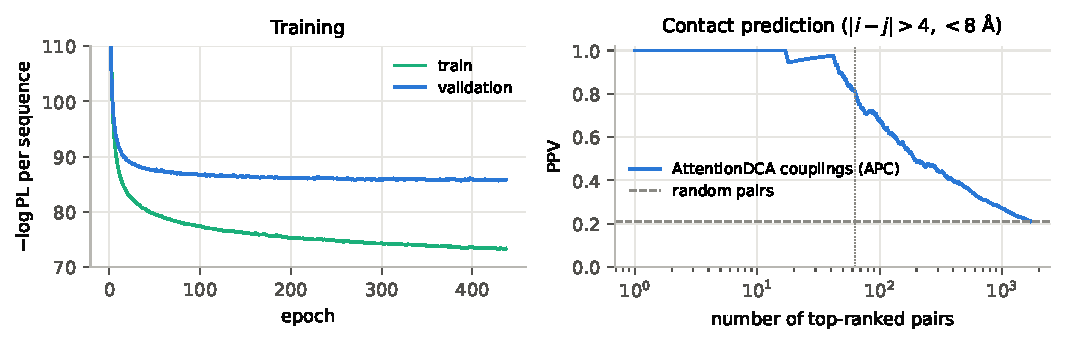
\includegraphics[width=\linewidth]{../outputs/figures/training_contacts.pdf}
\caption{Left: weighted $-\log\mathrm{PL}$ per sequence (training batches vs.\ validation split).
Right: contact-prediction precision of the ranked APC-corrected coupling norms; the vertical line marks $L$ pairs.}
\label{fig:train}
\end{figure}


%======================================================================
\section{Sampling and decorrelation}
%======================================================================

\paragraph{Implementation.} All chains are updated at once on the GPU: the conditional
logits of site $i$ for $C$ chains are a single $(C\times Lq)\cdot(Lq\times q)$ product. One
site-update per chain costs about $0.3\,\mu$s, against 0.6\,ms (NumPy) to 28\,ms (torch tensor) in the
original pure-Python loop, a speed-up of $10^3$--$10^5$. The original code also saved the state after
\emph{every single-site update} as a new sample, so consecutive ``sequences'' differed at
$\le1$ site. Here every sample is the final state of an independent chain.

\paragraph{Temperature.} Pseudo-likelihood fits the conditionals, not the global
normalisation, so the $\beta=1$ chain need not have the energy of natural sequences. Figure~\ref{fig:beta}
scans $\beta$ (3000 chains, 1000 sweeps). At $\beta=1$ the chains sit slightly above the natural
energy, and increasing $\beta$ trades diversity for sharper correlations. We report $\beta=1$
(the learned model as is) and $\beta^*=\BetaStar$, the value at which the mean energy of the samples
equals the reweighted mean energy of the \emph{training} set (\Etrain). $\beta^*$ is therefore chosen
without looking at the test set.

\paragraph{Decorrelation from the initial sequence.} Figure~\ref{fig:mixing} follows 1000 chains
started from training sequences and 1000 from uniformly random sequences over \StudySweeps\ sweeps.
\begin{itemize}\itemsep0pt
\item Random starts ($E\approx\Erandom$) fall into the family basin within about 20 sweeps and reach
      the same stationary energy as natural starts ($\EendRndOne$ vs.\ $\EendNatOne$ at $\beta=1$).
      The stationary state therefore does not depend on the start.
\item Chains started from natural sequences first rise in energy (natural sequences are more
      stable than typical samples at $\beta=1$), then fluctuate around the stationary mean.
\item The distance from the start reaches 90\% of its plateau after \SweepsNinetyOne\ sweeps. The plateau
      ($\HamEndOne$) is at or above the mean test--test distance ($\HamTestTest$): the chain
      forgets its seed entirely.
\item Stationary energy autocorrelation: $\tau_\text{int}=\TauOne$ sweeps at $\beta=1$ and $\TauStar$
      at $\beta^*$ (PLL: $\TauPOne$ and $\TauPStar$). Generation uses \BurnOne\ sweeps per chain
      ($\approx40\,\tau_\text{int}$), \NgenOne\ independent chains per temperature.
\item No chain ends in a degenerate gap-only state (0 of \NgenOne; $>90\%$ gaps is the filter
      applied to the natural MSA). Such a collapse \emph{did} occur (up to 40\% of chains) with an
      under-trained model (150 epochs, $H=32$), where the all-gap sequence was the energy
      minimum. It disappears once training converges.
\end{itemize}

\begin{figure}[h]\centering
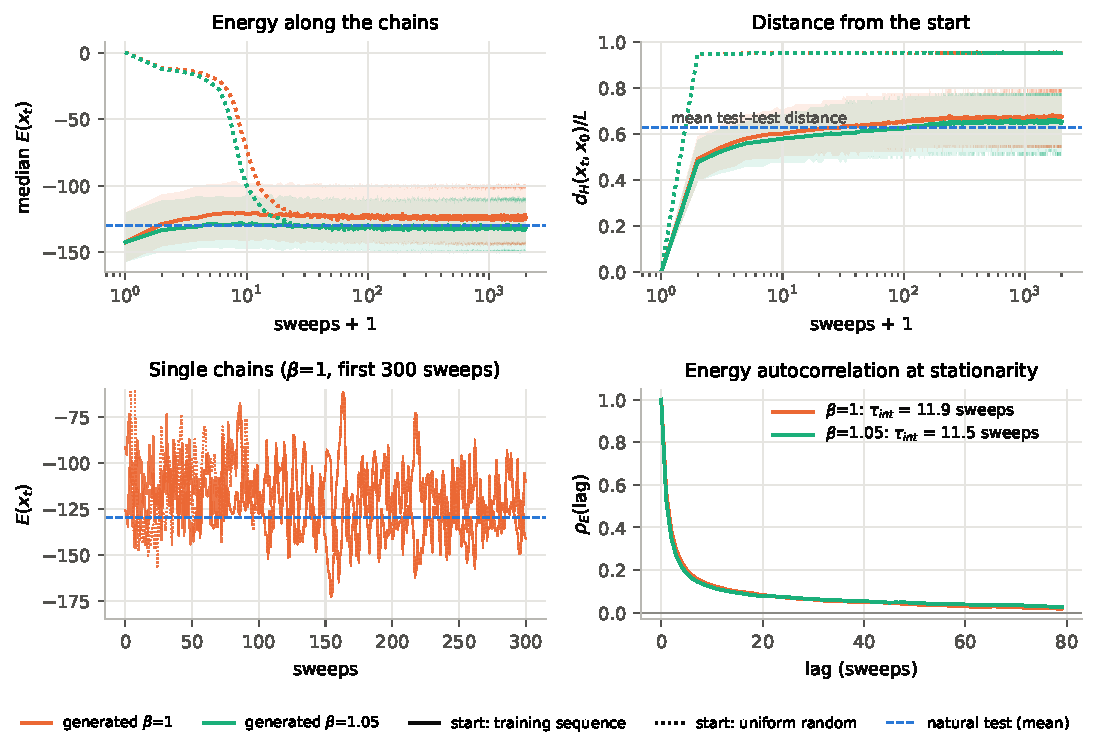
\includegraphics[width=\linewidth]{../outputs/figures/mixing.pdf}
\caption{Pseudo-likelihood sampling. (a) median energy (band: 10--90\% of chains from training
starts); (b) normalised Hamming distance to the starting sequence; (c) individual chains at
$\beta=1$ (solid: training start, dotted: random start); (d) chain-averaged energy
autocorrelation over the second half of the chains.}
\label{fig:mixing}
\end{figure}

\begin{figure}[h]\centering
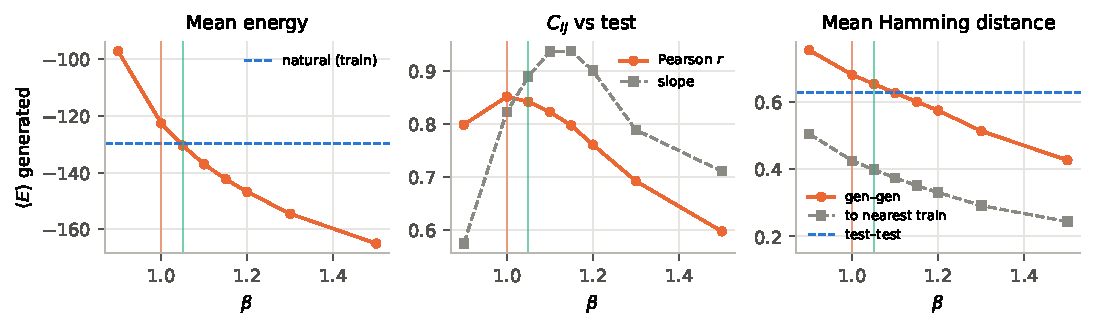
\includegraphics[width=\linewidth]{../outputs/figures/beta_scan.pdf}
\caption{Inverse-temperature scan (chains started from training sequences). Vertical lines mark
$\beta=1$ and $\beta^*=\BetaStar$. Right: mean pairwise distance among samples (gen--gen), mean
distance to the closest training sequence, and the natural test--test value.}
\label{fig:beta}
\end{figure}


%======================================================================
\section{Generated vs.\ natural sequences}\label{sec:gen}
%======================================================================

\paragraph{PCA (Fig.~\ref{fig:pca}).} The first two components of the one-hot test set
explain \PCone\% and \PCtwo\% of the variance. $k$-means with $k=\Kclust$ on the (PC1,\,PC2)
plane of the natural test set splits the family into two large clusters and one minor one
(the elbow of the within-cluster inertia sits at $k=3$). Writing $s_k$ for a cluster's share of
a set's total weight, a cluster counts as \emph{covered} when
$s^\text{gen}_k/s^\text{nat}_k\ge0.6$ for both temperatures. \NcovClust\ of the \Kclust\ clusters
are covered, holding \CovWeight\% of the natural test weight; the remaining minor cluster
(HscB-like J-domains) holds \ClTest\% of the natural test weight but only \ClOne\%
($\beta=1$) and \ClStar\% ($\beta^*$) of the samples. About one chain in ten \emph{starts} inside
it, so this is not a failure to reach the cluster: the model gives it too little stationary
weight. Over the covered region the agreement is good --- the 1-D Wasserstein distances to
the reweighted test distribution along PC1/PC2 are $\WPCaOne/\WPCbOne$ ($\beta=1$) and
$\WPCaStar/\WPCbStar$ ($\beta^*$), against $\WPCaProf/\WPCbProf$ for the independent-site model.

\begin{figure}[h]\centering
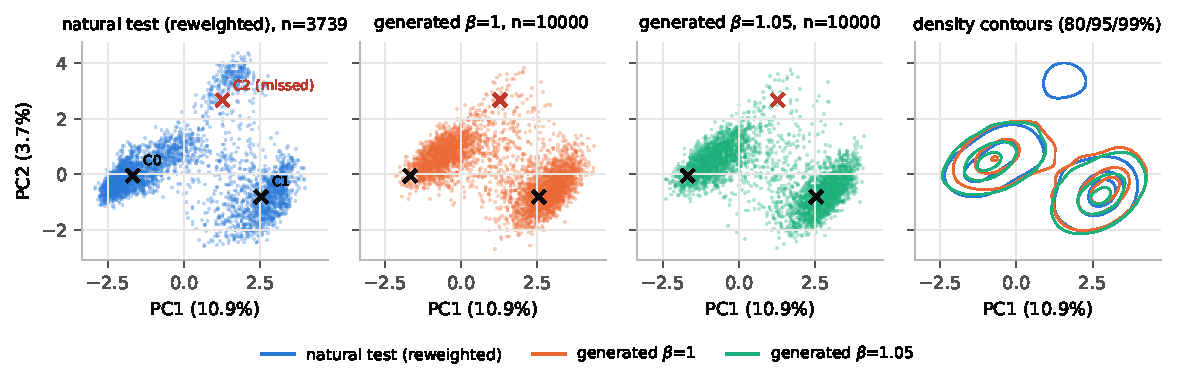
\includegraphics[width=\linewidth]{../outputs/figures/pca.pdf}
\caption{Test and generated sequences projected on the first two principal components of the
one-hot test alignment (PCA fitted on the test set only); each panel draws a random sample of
the points, the natural panel drawn with its reweighting weights. Crosses: $k$-means centres,
red for the cluster the samples miss. Right: densities of the full sets.}
\label{fig:pca}
\end{figure}

\paragraph{Why the minor cluster is missed: the model does not learn the priors.}
Table~\ref{tab:clusene} separates the two things that set a cluster's share of the samples.
The pseudo-likelihood of \emph{training} sequences is essentially the same in all three clusters
(\PLLmissTrain\ nats for \MissCl\ against \PLLcovTrain\ for the covered ones), so the model has
learned the local statistics of the minor sub-family about as well as everything else. Its
\emph{energy}, however, is not comparable at all: natural sequences of \MissCl\ score
\EmissTest\ on the test set and \EmissTrain\ on the training set, roughly \EgapMiss\ units above
the covered clusters (\EcovTest\ and \EcovTrain). Since the stationary weight of a basin is set by
its free energy, that offset is what starves the cluster: the measured free-energy error is
$\Delta F=-\ln(s^\text{gen}/s^\text{nat})=\dFmiss$ nats for \MissCl, i.e.\ the sampler gives it
\dFmissFac\ of its natural weight, against $|\Delta F|\le0.23$ for the other two.

This is the expected failure mode of this objective. Maximising the pseudo-likelihood constrains
the conditionals $p(x_i\mid\bm x_{\setminus i})$ --- purely local quantities --- and never the
global normalisation, so nothing in the loss asks the model to reproduce how \emph{much} total
probability mass each sub-family carries. The model has no fields and no mixture component to hold
such a prior; the relative weight of the basins is only an indirect consequence of the couplings.
Reweighting is \emph{not} the culprit here, as one might suspect: \MissCl\ is only
\RawShareMiss\% of the raw training sequences but \ClTrain\% of the reweighted ones, so the weights
already nearly double its influence and the model still undershoots to \ClOne\%. What the model
misses is the target it was actually given. The result is a model that describes
every sub-family correctly and populates them in the wrong proportion. It is also why the
independent-site baseline distributes its samples as $(0.02,0.10,0.88)$ against the natural
$(0.14,0.39,0.47)$: cluster identity is a covariation effect, and a model without couplings
collapses onto the single dominant mode.

\begin{table}[h]\centering\small
\begin{tabular}{crrrrrrr}
\toprule
cluster & \multicolumn{2}{c}{weight share} & \multicolumn{2}{c}{$\langle E\rangle$ natural} & \multicolumn{2}{c}{$\langle\log\mathrm{PL}\rangle$ natural} & $\Delta F$ \\
\cmidrule(lr){2-3}\cmidrule(lr){4-5}\cmidrule(lr){6-7}
 & natural & generated & test & train & test & train & (nats) \\
\midrule
C0$^{\dagger}$ & 0.141 & 0.051 & -119.5 & -122.6 & -80.5 & -71.8 & +1.01 \\
C1 & 0.387 & 0.352 & -134.0 & -134.5 & -76.8 & -71.1 & +0.09 \\
C2 & 0.473 & 0.597 & -133.5 & -137.2 & -79.7 & -71.0 & -0.23 \\
\bottomrule
\end{tabular}
\caption{Per-cluster diagnosis of the sampling weights ($\beta=1$). Weight shares and
$\langle\cdot\rangle$ use the reweighting weights for the natural sets. $\Delta F=-\ln(
s^\text{gen}/s^\text{nat})$ is the model's free-energy error for the cluster, in nats.
$^{\dagger}$: the cluster the sampler misses. The conditionals are fitted equally well everywhere
($\langle\log\mathrm{PL}\rangle$ on train), but the energy of \MissCl\ is far higher, so its
Boltzmann weight is far too small.}
\label{tab:clusene}
\end{table}

\paragraph{Statistics restricted to the covered clusters (Fig.~\ref{fig:statsclust},
Table~\ref{tab:clusters}).} To separate ``the model distorts the covariation'' from ``the model
misses one sub-family'', the whole comparison is repeated with \emph{both} sets restricted to the
covered clusters (natural: \NtestCov\ sequences, $M_\text{eff}=\MeffTestCov$; weights recomputed
inside the subset). The correlation agreement rises from $\rCOne$ to $\rCcovOne$ at $\beta=1$ and
from $\rCStar$ to $\rCcovStar$ at $\beta^*$, while the train-vs-test ceiling barely moves
($\rCtrain\to\rCtrainCov$): inside the modes it populates, the model is close to the
finite-sampling limit, and the missed sub-family accounts for most of the residual gap. On the
strongest 1\% of correlations the restricted agreement is $\rCcovTopOne$ / $\rCcovTopStar$, with
the $\beta^*$ slope at $\sCcovStar$.

\begin{figure}[h]\centering
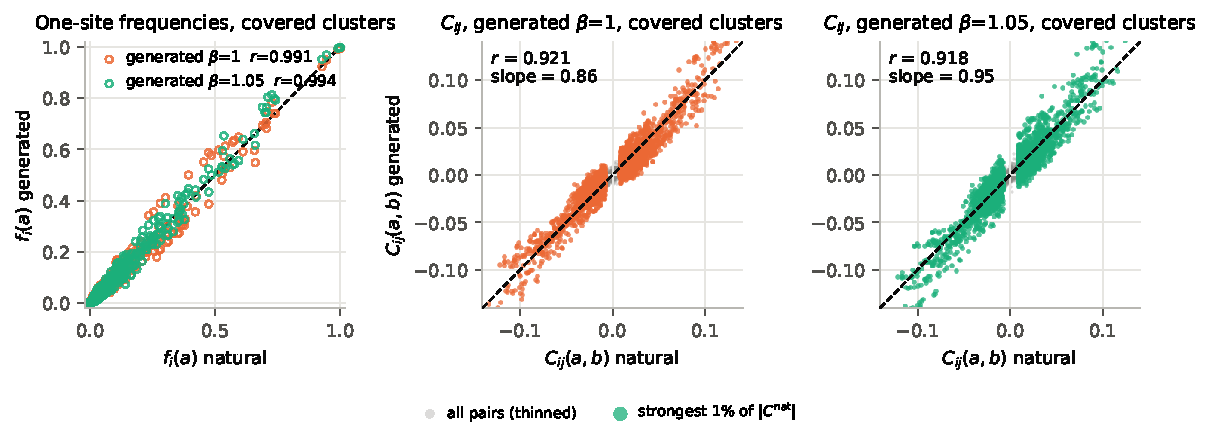
\includegraphics[width=\linewidth]{../outputs/figures/freqs_corr_clusters.pdf}
\caption{As Fig.~\ref{fig:stats}, with natural and generated sets both restricted to the
covered PCA clusters.}
\label{fig:statsclust}
\end{figure}

\begin{table}[h]\centering\small
\begin{tabular}{llcccc}
\toprule
statistic & set vs.\ natural (covered clusters) & Pearson $r$ & Spearman $\rho$ & slope & RMSE \\
\midrule
$f_i(a)$ & generated, $\beta=1$ & 0.991 & 0.970 & 0.98 & 0.0153 \\
 & generated, $\beta^*=1.05$ & 0.996 & 0.969 & 1.03 & 0.0118 \\
 & natural train (ceiling) & 0.998 & 0.980 & 0.98 & 0.0079 \\
 & independent-site model & 0.993 & 0.973 & 0.95 & 0.0144 \\
\midrule
$C_{ij}(a,b)$ & generated, $\beta=1$ & 0.918 & 0.179 & 0.82 & 0.0012 \\
 & generated, $\beta^*=1.05$ & 0.918 & 0.199 & 0.91 & 0.0013 \\
 & natural train (ceiling) & 0.941 & 0.345 & 0.87 & 0.0010 \\
 & independent-site model & -0.013 & 0.060 & -0.00 & 0.0031 \\
\midrule
$C_{ij}$, top 1\% & generated, $\beta=1$ & 0.961 & 0.919 & 0.87 & 0.0084 \\
 & generated, $\beta^*=1.05$ & 0.961 & 0.919 & 0.97 & 0.0083 \\
 & natural train (ceiling) & 0.979 & 0.938 & 0.91 & 0.0061 \\
 & independent-site model & -0.031 & -0.035 & -0.00 & 0.0296 \\
\bottomrule
\end{tabular}
\caption{Statistics restricted to the covered PCA clusters (\CovWeight\% of the natural test
weight). Compare with Table~\ref{tab:stats}, which uses the full sets.}
\label{tab:clusters}
\end{table}

\paragraph{One- and two-site statistics (Fig.~\ref{fig:stats}, Table~\ref{tab:stats}).}
Site frequencies are reproduced almost exactly ($r=\rFOne$). The connected correlations reach
$r=\rCOne$ at $\beta=1$ and $r=\rCStar$ at $\beta^*$, against a finite-sample ceiling of
$\rCtrain$ (train vs.\ test) and $\rCprof$ for the independent-site model, which matches
$f_i$ equally well. The regression slope shows that $\beta=1$ under-estimates the correlation
amplitudes ($\sCOne$), and $\beta^*$ corrects most of this ($\sCStar$, against a ceiling of
$\sCtrain$). Note that $r$ and the slope measure different things and are related by
$\text{slope}=r\,\sigma_\text{gen}/\sigma_\text{nat}$: $r$ is the tightness of the relation and is
blind to a uniform rescaling, the slope is the amplitude. Neither should be compared to 1 naively
--- the natural $C_{ij}$ carry sampling noise, which attenuates any least-squares slope. A
half-split of the test set puts their reliability at \Crel, and dividing by it gives disattenuated
slopes \sCdisOne\ ($\beta=1$), \sCdisStar\ ($\beta^*$) and \sCdisTrain\ (ceiling).
The low Spearman values on $C_{ij}$ are expected: most of the \NCij\ entries
are sampling noise around zero, so their ranks carry little information; on the strongest 1\%
of the entries the rank agreement is high as well (Table~\ref{tab:stats}).

\begin{figure}[h]\centering
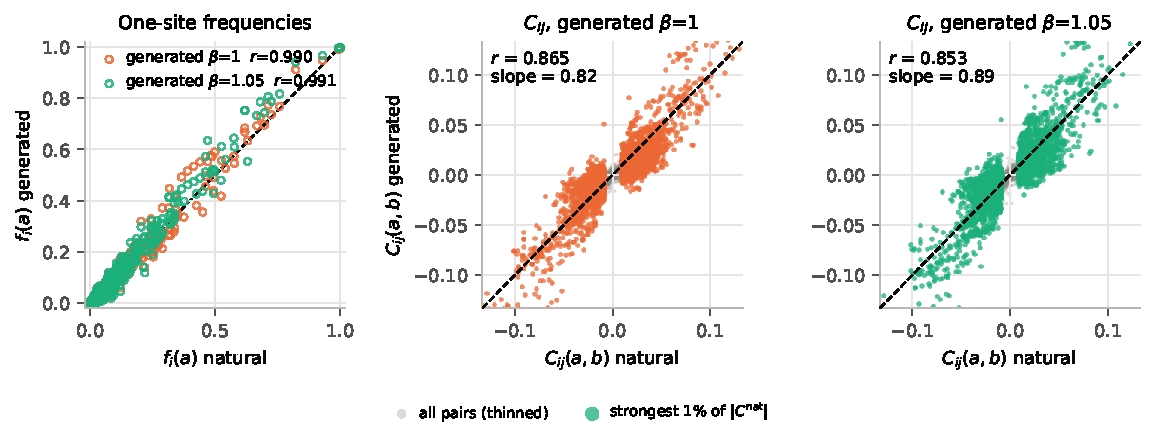
\includegraphics[width=\linewidth]{../outputs/figures/freqs_corr.pdf}
\caption{Generated vs.\ natural (reweighted test) one-site frequencies (\NfOne\ values) and
connected correlations. The $C_{ij}$ panels show the strongest 1\% of $|C^\text{nat}_{ij}(a,b)|$
in colour over a thinned grey sample of all \NCij\ entries. Dashed: identity.}
\label{fig:stats}
\end{figure}

\begin{table}[h]\centering\small
\begin{tabular}{llcccc}
\toprule
statistic & set vs.\ natural test & Pearson $r$ & Spearman $\rho$ & slope & RMSE \\
\midrule
$f_i(a)$ & generated, $\beta=1$ & 0.990 & 0.972 & 1.01 & 0.0160 \\
 & generated, $\beta^*=1.05$ & 0.992 & 0.970 & 1.06 & 0.0165 \\
 & natural train (ceiling) & 0.998 & 0.983 & 0.99 & 0.0070 \\
 & independent-site model & 0.998 & 0.982 & 0.99 & 0.0072 \\
\midrule
$C_{ij}(a,b)$ & generated, $\beta=1$ & 0.871 & 0.193 & 0.78 & 0.0015 \\
 & generated, $\beta^*=1.05$ & 0.859 & 0.209 & 0.85 & 0.0016 \\
 & natural train (ceiling) & 0.944 & 0.377 & 0.88 & 0.0010 \\
 & independent-site model & -0.005 & 0.058 & -0.00 & 0.0030 \\
\midrule
$C_{ij}$, top 1\% & generated, $\beta=1$ & 0.918 & 0.880 & 0.84 & 0.0113 \\
 & generated, $\beta^*=1.05$ & 0.908 & 0.865 & 0.93 & 0.0123 \\
 & natural train (ceiling) & 0.981 & 0.949 & 0.91 & 0.0057 \\
 & independent-site model & -0.009 & -0.022 & -0.00 & 0.0283 \\
\bottomrule
\end{tabular}
\caption{Agreement of generated statistics with the natural test set (natural sets reweighted,
generated sets uniform). ``Top 1\%'': the 1\% largest $|C^\text{test}_{ij}(a,b)|$.}
\label{tab:stats}
\end{table}

\paragraph{Diversity and novelty (Fig.~\ref{fig:ham}, Table~\ref{tab:ham}).}
\begin{itemize}\itemsep0pt
\item \textbf{Generated vs.\ test.} The closest test sequence lies on average at \HamGTOne\ ($\beta=1$) and
      \HamGTStar\ ($\beta^*$). Two natural references bound this: a test sequence's closest
      \emph{other} test sequence sits at \HamTestNN\ and its closest \emph{training} sequence at
      \HamTestTrain. Natural sequences therefore have much closer natural neighbours than the
      generated ones do --- the samples are new sequences, not near-copies.
\item \textbf{Generated vs.\ train.} There is no memorisation: the mean distance to the closest training
      sequence is \HamGTrOne\ (5\% quantile \HamGTrMinOne) and every sample is distinct
      (\UniqOne\% unique).
\item \textbf{Generated vs.\ generated.} The all-pairs distribution (mean \HamGGOne\ at $\beta=1$, \HamGGStar\
      at $\beta^*$) sits on top of the test--test distribution (\HamTestTest), without the
      left tail of near-identical natural pairs (phylogenetic redundancy removed by the
      weights). The samples are therefore neither collapsed onto a few modes nor spread too thin.
\end{itemize}

\begin{figure}[h]\centering
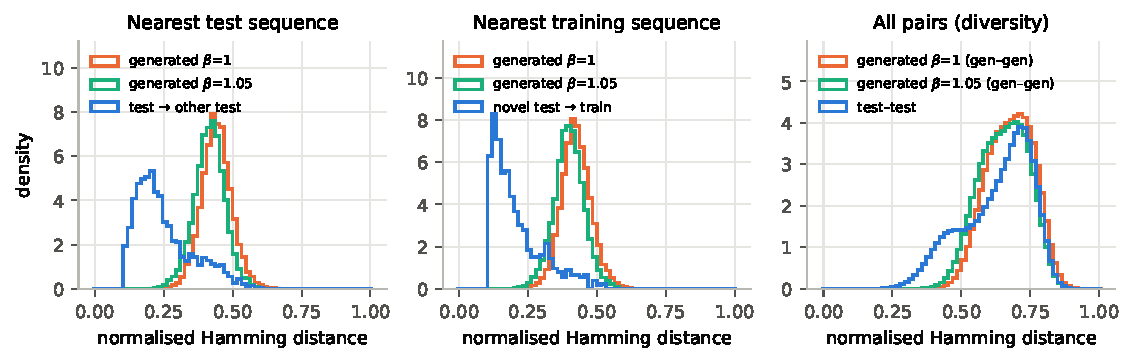
\includegraphics[width=\linewidth]{../outputs/figures/hamming.pdf}
\caption{Normalised Hamming distances; triangles mark means. Each panel carries a different
blue natural reference, and each answers a different question.
\textbf{(a)} nearest-neighbour distance \emph{into the test set}: for the generated sets, how far
each sample is from the closest natural test sequence; the blue curve is the same quantity for a
test sequence against the \emph{other} test sequences (leave-one-out), i.e.\ how close natural
relatives normally are. Its spike near zero is the family's phylogenetic redundancy.
\textbf{(b)} nearest-neighbour distance \emph{into the training set} --- the memorisation check.
Blue is the held-out test set measured the same way, which is the strongest ``legitimate''
proximity to training data a genuine J-domain shows.
\textbf{(c)} all pairwise distances \emph{inside} one set (3000 sequences per set): the spread of
the set itself. Blue is the natural test set; the dotted grey curve is generated-vs-test, which
lies on top of the generated curve when the two sets occupy the same region of sequence space.}
\label{fig:ham}
\end{figure}

\begin{table}[h]\centering\small
\begin{tabular}{lcccc}
\toprule
distance (normalised by $L$) & mean & median & 5\% quantile & $=0$ \\
\midrule
gen ($\beta=1$) $\to$ nearest test & 0.437 & 0.444 & 0.333 & 0.0\% \\
gen ($\beta=1$) $\to$ nearest train & 0.420 & 0.413 & 0.317 & 0.0\% \\
gen ($\beta=1$) $\to$ nearest other gen & 0.430 & 0.429 & 0.349 & 0.0\% \\
gen--gen, all pairs ($\beta=1$) & 0.679 & 0.683 & 0.540 & 0.0\% \\
gen--test, all pairs ($\beta=1$) & 0.666 & 0.683 & 0.492 & 0.0\% \\
\midrule
gen ($\beta^*=1.05$) $\to$ nearest test & 0.405 & 0.413 & 0.302 & 0.0\% \\
gen ($\beta^*=1.05$) $\to$ nearest train & 0.389 & 0.397 & 0.286 & 0.0\% \\
gen ($\beta^*=1.05$) $\to$ nearest other gen & 0.394 & 0.397 & 0.317 & 0.0\% \\
gen--gen, all pairs ($\beta^*=1.05$) & 0.650 & 0.651 & 0.508 & 0.0\% \\
gen--test, all pairs ($\beta^*=1.05$) & 0.639 & 0.651 & 0.460 & 0.0\% \\
\midrule
test $\to$ nearest other test & 0.116 & 0.079 & 0.016 & 0.0\% \\
test $\to$ nearest train & 0.179 & 0.175 & 0.032 & 0.0\% \\
novel test $\to$ nearest train & 0.179 & 0.175 & 0.032 & 0.0\% \\
test--test, all pairs & 0.598 & 0.635 & 0.365 & 0.0\% \\
\bottomrule
\end{tabular}
\caption{Hamming-distance summary; ``$=0$'' is the fraction of exact copies.}
\label{tab:ham}
\end{table}

\paragraph{Energy of the samples (Fig.~\ref{fig:energy}).} The reweighted mean energy of the test
sequences is \Etest\ (unweighted \Eunw). Samples at $\beta=1$ have mean \EgenOne\ (Wasserstein
distance to test \WEOne); at $\beta^*$ the distribution lies on top of the natural one (\EgenStar,
distance \WEStar, independent-site model \WEprof). Per-site pseudo-log-likelihoods show the same
ordering: independent-site $\ll$ $\beta=1$ $<$ $\beta^*$ $\lesssim$ natural.

\begin{figure}[h]\centering
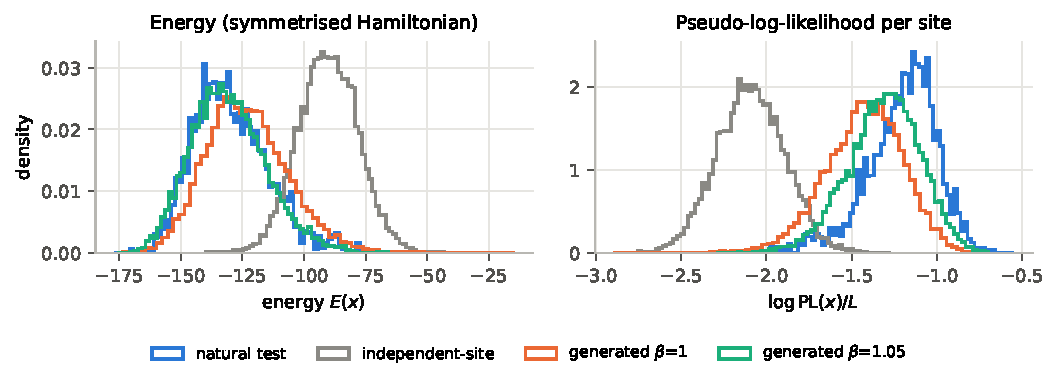
\includegraphics[width=\linewidth]{../outputs/figures/energy_dist.pdf}
\caption{Distribution of the energy $E(\bm x)$ and of $\log\mathrm{PL}(\bm x)/L$ under the trained model.}
\label{fig:energy}
\end{figure}


%======================================================================
\section{Effect of the split}\label{sec:compare}
%======================================================================
Everything above uses the sequence-disjoint split of \S\ref{sec:data}. Running the identical
pipeline on the supplied species split (\CmpMtrain\ train / \CmpMtest\ test, \CmpPctCopies\% of
the test set copied from the training set) gives the numbers in the second column below. The
two differ in the direction one expects: the shipped split makes the model look better on the
held-out likelihood, because most of its ``test'' sequences were seen during training.

\begin{center}\small
\begin{tabular}{lcc}
\toprule
 & sequence-disjoint (this work) & supplied species split \\
\midrule
train / test sequences & \Mtrain\ / \Mtest & \CmpMtrain\ / \CmpMtest \\
test sequences copied from train & 0\% & \CmpPctCopies\% \\
validation $-\log\mathrm{PL}$ per sequence & \ValNLPL & \CmpValNLPL \\
test $-\log\mathrm{PL}$ per sequence & \NLPLtest & \CmpNLPLtest \\
\quad on its non-copied test sequences & --- & \CmpNLPLnovel \\
contact PPV at $L/2$ & \PPVLhalf & \CmpPPVLhalf \\
$r(f_i)$, $\beta=1$ & \rFOne & \CmprFOne \\
$r(C_{ij})$, $\beta=1$ & \rCOne & \CmprCOne \\
\quad ceiling (train vs.\ test) & \rCtrain & \CmprCtrain \\
\quad restricted to covered clusters & \rCcovOne & \CmprCcovOne \\
generated $\to$ nearest train, $\beta=1$ & \HamGTrOne & \CmpHamGTrOne \\
\bottomrule
\end{tabular}
\end{center}

The generative metrics themselves are barely affected --- the model learns nearly the same
distribution either way --- but the \emph{interpretation} of the likelihood numbers changes
completely, and only the disjoint split supports a claim of generalisation.

%======================================================================
\section{Conditioning generation on PCA coordinates}\label{sec:cond}
%======================================================================
An earlier version of this project steered generation by appending the discretised PCA coordinates
to every sequence as two extra Potts sites and amplifying their couplings by a factor
$\beta_\mathrm{PCA}$ at sampling time; steering only began around $\beta_\mathrm{PCA}\approx10$, and
beyond it the samples drifted past the target and lost the HPD motif. Here we test two
alternatives, both built on one exact property of the PCA used throughout this report. The full
study, including a slower derivation, is in the companion note \texttt{conditional.pdf}.

\paragraph{A PCA coordinate is an exact Potts term.} The PCA is fitted on one-hot vectors, so once
fitted a coordinate is a projection, and because a one-hot sequence has a single $1$ per site the
projection reduces to one table entry per site:
\begin{equation}
\mathrm{PC}_c(\bm x)=\sum_{i}V_c(i,x_i)-m_c .
\end{equation}
Squaring a sum of per-site terms produces per-site and pairwise terms, so the harmonic restraint
\begin{equation}
E_\lambda(\bm x)=E(\bm x)+\frac{\lambda}{2}\sum_c\big(\mathrm{PC}_c(\bm x)-t_c\big)^2
\label{eq:restraint}
\end{equation}
is itself a Potts energy, with coupling correction $\Delta J_{ij}(a,b)=-\lambda\sum_cV_c(i,a)V_c(j,b)$
and a field linear in the target $\bm t$. Its Boltzmann distribution is $p(\bm x)$ times a Gaussian
window of width $1/\sqrt\lambda$ around $\bm t$, i.e.\ exactly the posterior of $\bm x$ given a noisy
measurement $\mathrm{PC}(\bm x)\approx\bm t$.

\paragraph{Two methods.} \textbf{C1} adds \eqref{eq:restraint} to the trained model at sampling time:
each site update also scores how far each candidate letter would put the coordinate from $\bm t$.
Nothing is retrained. \textbf{C3} learns the conditional instead: fields
$h_i(a\mid\bm z)=\sum_fW_f(i,a)\phi_f(\bm z)$ with $\phi=(1,u_1,u_2,u_1^2,u_2^2,u_1u_2)$ ($\bm u$ the
standardised coordinates) are trained jointly with the couplings by conditional pseudo-likelihood on
pairs $(\bm x,\mathrm{PC}(\bm x)+\sigma\bm\epsilon)$, then sampled at $\bm z=\bm t$. Trained on
coordinates blurred by $\sigma$, C3 is fitted to the same distribution C1 writes down with
$\lambda=1/\sigma^2$; we use $\sigma=1,0.5,0.25$ to match $\lambda=1,4,16$. Optionally a gain $\kappa$
multiplies the $\bm z$-dependent field at sampling time --- the analogue of $\beta_\mathrm{PCA}$.

\paragraph{Setup.} Targets are the three cluster centres of \S\ref{sec:gen} (\MissCl, the
under-sampled HscB-like group, and the two others). For each method, target and setting, $3000$
chains start from random training sequences and run $500$ sweeps; the restrained chains converge in
$50$--$100$ sweeps. Quality is measured against the natural test sequences of the target cluster,
with every pool (including the natural ceiling) evaluated at the same size of $3000$ because $C_{ij}$
estimates are noisy. Both methods use the same field-free model, trained with longer patience
(best epoch \EpBase\ instead of \EpClean).

\paragraph{A caveat on mode weights uncovered on the way.} That longer-trained model has a slightly
better validation pseudo-likelihood (\ValBase\ vs \ValClean\ nats per sequence) but samples the
three clusters in proportions \ShareBasep\ (C0/C1/C2, \%) instead of \ShareClean\ for the model of
the previous sections (natural \ShareNat). Retraining the earlier model reproduces its couplings bit
for bit, so the only difference is $294$ epochs of training: the C1/C2 balance moved by $2.7$ nats of
free energy for $0.2$ nats of pseudo-likelihood. The good coverage of the two major clusters reported
above is therefore a property of that checkpoint, not a robust property of pseudo-likelihood
training; the deficit of \MissCl\ is present in every model trained.

\begin{figure}[t]\centering
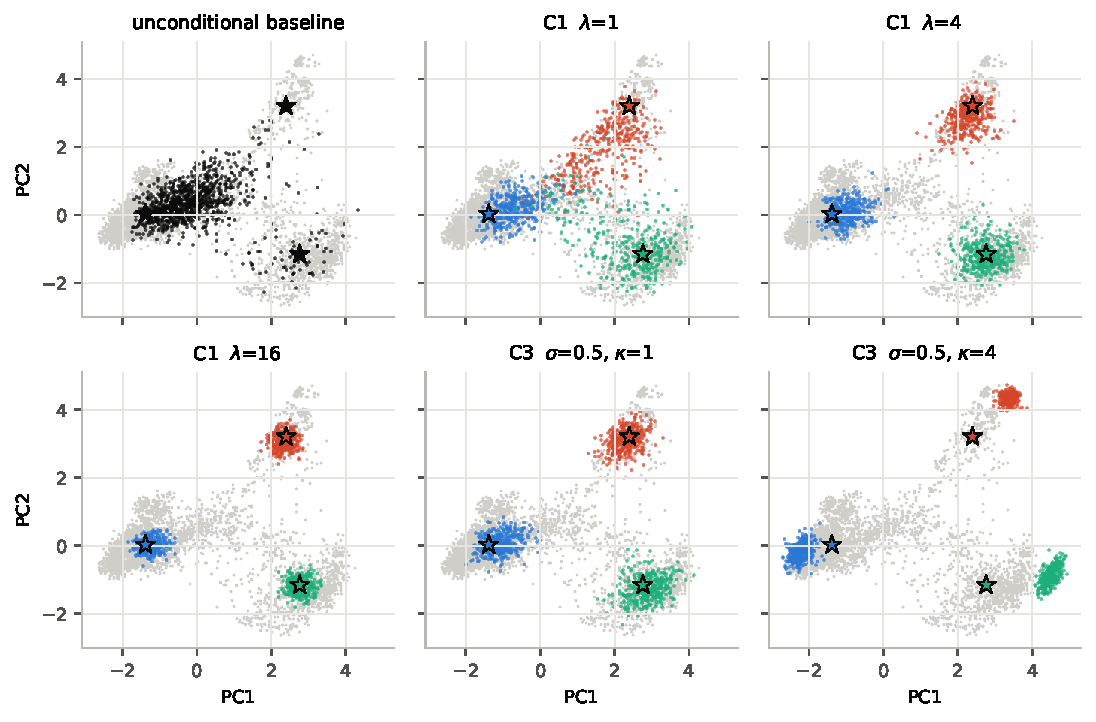
\includegraphics[width=0.84\linewidth]{../outputs/figures/cond_pca.pdf}
\caption{Conditioned samples in the PCA plane (grey: natural test). Stars: targets; points are
coloured by the target they were aimed at. Top left: unconditional sampling, which visits C1 almost
exclusively. Bottom right: C3 with its target field amplified ($\kappa=4$) --- every pool lands
beyond its target.}
\label{fig:condpca}
\end{figure}

\begin{table}[t]\centering\small\setlength{\tabcolsep}{4pt}
\begin{tabular}{lccccc}
\toprule
 & in target (\%) & distance & $r(C_{ij})$ & HPD (\%) & diversity \\
\midrule
unconditional baseline & 5/86/10 & 3.9/1.5/3.3 & 0.16/0.42/0.34 & 99/99/99 & 0.62/0.62/0.62 \\
rejection from baseline & 100/100/100 & 1.8/1.2/1.2 & 0.25/0.50/0.49 & 97/99/98 & 0.69/0.59/0.68 \\
\midrule
C1 $\lambda{=}1$ & 80/100/88 & 1.6/0.9/1.0 & 0.44/0.47/0.57 & 96/99/98 & 0.70/0.56/0.65 \\
C1 $\lambda{=}4$ & 100/100/100 & 0.6/0.5/0.5 & 0.46/0.39/0.60 & 96/99/99 & 0.64/0.52/0.62 \\
C1 $\lambda{=}16$ & 100/100/100 & 0.3/0.3/0.3 & 0.37/0.30/0.54 & 96/99/98 & 0.61/0.48/0.61 \\
\midrule
C3 $\sigma{=}1$ & 100/100/100 & 0.7/0.9/0.7 & 0.47/0.48/0.64 & 100/99/99 & 0.63/0.56/0.62 \\
C3 $\sigma{=}0.5$ & 100/100/100 & 0.4/0.5/0.5 & 0.38/0.40/0.60 & 100/100/100 & 0.57/0.52/0.61 \\
C3 $\sigma{=}0.25$ & 100/100/100 & 0.3/0.3/0.4 & 0.33/0.34/0.56 & 100/99/99 & 0.56/0.48/0.60 \\
\midrule
C3 $\sigma{=}0.5$, $\kappa{=}4$ & 100/100/100 & 1.5/0.9/1.8 & 0.12/0.18/0.29 & 100/100/92 & 0.29/0.31/0.55 \\
C3 $\sigma{=}0.5$, $\kappa{=}8$ & 100/100/100 & 1.6/1.2/1.8 & 0.08/0.08/0.12 & 100/100/56 & 0.16/0.21/0.40 \\
\midrule
natural (ceiling) & 100/100/100 & 1.0/1.3/0.8 & 0.66/0.63/0.75 & 100/100/99 & 0.67/0.60/0.64 \\
\bottomrule
\end{tabular}

\caption{Conditioning on each of the three cluster centres; each entry lists C0/C1/C2. In target:
fraction of samples landing in the target cluster. Distance: mean $\|\mathrm{PC}-\bm t\|$.
$r(C_{ij})$: against the natural test sequences of the target cluster. HPD: fraction retaining the
J-domain HPD motif. Diversity: mean pairwise Hamming distance within the pool. Rejection keeps the
unconditional samples that fall in the cluster ($496$, $3000$, $948$ sequences). Ceiling: $3000$
natural training sequences of the cluster.}
\label{tab:cond}
\end{table}

\paragraph{C1 steers to every target, including the neglected one, and keeps the protein.} Without
the restraint, $5\%$ of the chains reach \MissCl; from $\lambda=4$ on, all of them do
(Table~\ref{tab:cond}, Figure~\ref{fig:condpca}). The distance to the target falls as
$1/\sqrt\lambda$, the width of the Gaussian window, and responds monotonically to $\lambda$. The HPD
motif is retained in $96$--$99\%$ of samples at every $\lambda$. The covariation agreement peaks at
$\lambda\approx1$--$4$ (e.g.\ $r(C_{ij})=\ConeALfourrC$ for C0 and $0.60$ for C2 at $\lambda=4$,
ceilings \CeilA\ and \CeilC) and decreases for stiffer restraints, mainly because a window much
narrower than a natural cluster (radius ${\sim}1$) samples the cluster's centre and loses its
internal variation. Rejection sampling, the exact conditional, needs $10\,000$ unconditional samples
to produce $496$ in C0; C1 at $\lambda=4$ produces C0 sequences of the same energy (\ConeALfourE\ vs
$-106.0$), as expected if it samples the model's own conditional. That energy is $14$ units above the
natural C0 sequences (\NatEA): C1 reaches the neglected region but inherits the model's view of it.

\paragraph{C3 matches C1 at $\lambda=1/\sigma^2$, and does better on the neglected cluster.} At
$\kappa=1$ C3 lands on target with the accuracy and quality of C1 at the matching stiffness
(Table~\ref{tab:cond}), as the equivalence above predicts. The one systematic difference is
\MissCl: C3 gets there at weak conditioning where C1 stops short (distance $0.74$ vs $1.59$ at
$\sigma=1$/$\lambda=1$), and its C0 sequences have lower energy (\CthreeAsHKoneE\ vs \ConeALfourE),
closer to the natural ones. C1 reweights the unconditional model, which carries the free-energy
error of Table~\ref{tab:clusene}; C3 learned the conditional from data and does not inherit it.

\paragraph{Amplifying the target field reproduces the earlier failure.} With $\kappa=2,4,8$ the samples
overshoot the target by up to $1.5$ PC units, diversity collapses towards copies of a single
sequence ($0.16$ for C0 at $\kappa=8$), $r(C_{ij})$ drops to $0.1$, and for C2 the HPD motif is lost in
$44\%$ of the samples. The cause follows from the expansion of \eqref{eq:restraint}: the exact
conditional pairs a field that pushes towards $\bm t$ with a coupling term that holds the coordinate
\emph{at} $\bm t$; $\kappa$ (like $\beta_\mathrm{PCA}$) amplifies the push without the spring. This is
the ``drifts past the target, loses the HPD motif'' behaviour of the earlier study, now explained.

\begin{figure}[t]\centering
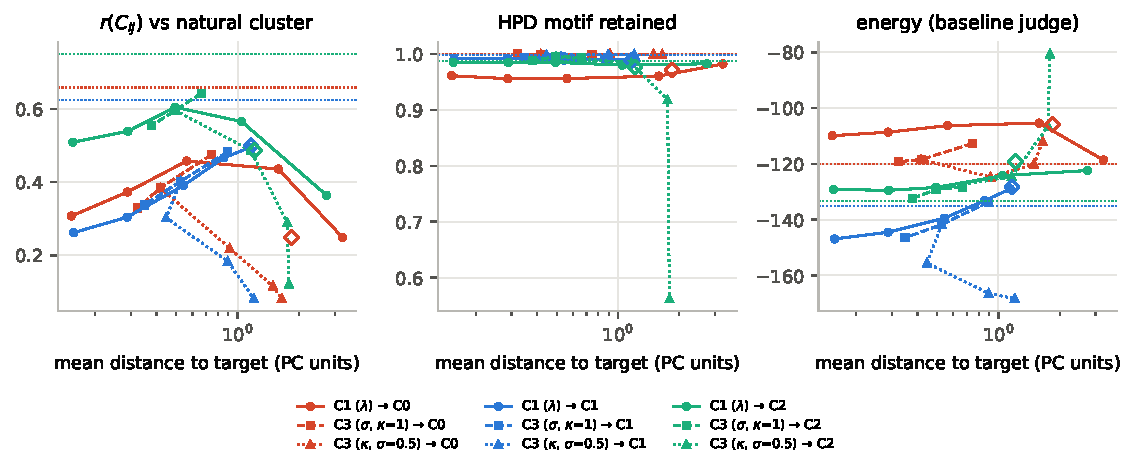
\includegraphics[width=\linewidth]{../outputs/figures/cond_tradeoff.pdf}
\caption{Accuracy--quality trade-off per method (line style) and target (colour). Solid circles: C1,
$\lambda=0.25\to64$ (right to left). Dashed squares: C3 at $\kappa=1$, $\sigma=1\to0.25$. Dotted
triangles: C3 at $\sigma=0.5$, $\kappa=1\to8$. Open diamonds: rejection. Dotted horizontal lines:
natural ceiling ($r(C_{ij})$) or natural cluster value (HPD, energy under the baseline model).}
\label{fig:condtrade}
\end{figure}


%======================================================================
\section{Summary and caveats}
%======================================================================

\begin{itemize}\itemsep1pt
\item \textbf{Data.} The supplied split is species-disjoint but not sequence-disjoint
      (\CmpPctCopies\% verbatim copies), so it cannot measure generalisation. The split used here
      clusters the full pool at \SplitIdent\% identity and moves whole clusters to one side
      (\Mtrain\ / \Mtest\ sequences, no exact copies, median distance \CleanNNmed\ to the nearest
      training sequence).
\item \textbf{Model.} The attention-factorised Potts model ($H=\Hbest$, $d=\dbest$) predicts contacts
      well (PPV \PPVLhalf\ at $L/2$) and keeps a \NLPLgapPct\% pseudo-likelihood gap to genuinely
      unseen sequences.
\item \textbf{Sampling.} The vectorised sampler is $10^3$--$10^5\times$ faster than the original code and
      decorrelates from its seed in about \SweepsNinetyOne\ sweeps ($\tau_\text{int}=\TauOne$). Samples are
      end-points of independent chains after \BurnOne\ sweeps ($\approx40\,\tau_\text{int}$).
\item \textbf{Generation quality.} $r(f_i)=\rFOne$ and $r(C_{ij})=\rCOne$--$\rCStar$ against the
      \rCtrain\ ceiling, rising to $\rCcovOne$--$\rCcovStar$ (ceiling $\rCtrainCov$) on the modes the
      sampler populates. The samples are novel and as diverse as natural sequences.
      $\beta^*=\BetaStar$ restores the correlation amplitude and the natural energy level at a
      small cost in diversity.
\item \textbf{Conditioning.} Because a PCA coordinate is an exact Potts term, a harmonic restraint
      added at sampling time (C1) steers generation to any cluster, including the neglected one
      ($5\%\to100\%$ of chains in it at $\lambda\ge4$), with the HPD motif kept in $\ge96\%$ of samples
      and the best correlation agreement at $\lambda\approx1$--$4$. A learned conditional field (C3)
      matches it at $\lambda=1/\sigma^2$ and is better on the neglected cluster; amplifying its field
      reproduces the over-steering of the earlier appended-coordinate approach.
\item \textbf{Limitations.}
      (i) PL training does not constrain the global normalisation, hence the $\beta$ offset.
      (ii) The attention couplings are asymmetric, so the PL chain is only approximately Boltzmann.
      (iii) The HscB-like sub-family is under-sampled (\ClOne\% vs.\ \ClTest\%) because
      pseudo-likelihood fits conditionals and not the relative masses of the basins: the model
      learns that sub-family's local statistics as well as any other
      ($\langle\log\mathrm{PL}\rangle$ on train \PLLmissTrain\ vs.\ \PLLcovTrain) but puts its
      energy \EgapMiss\ units too high, a free-energy error of \dFmiss\ nats. Explicit per-site
      fields do not fix it (tested in \texttt{conditional.pdf}: the sub-family stays at $5\%$); the
      balance between basins is also sensitive to when training stops (\S\ref{sec:cond}).
      Conditioning reaches the sub-family on demand (previous item); drawing targets from the natural
      distribution of coordinates and sampling conditionally would restore its weight by construction.
      (iv) The split removes only exact copies, so \CleanPctNear\% of the test set still lies
      within \SplitThresh\ of a training sequence; the held-out likelihood is a fair measure of
      generalisation to unseen sequences, not to unseen sub-families.
\end{itemize}
Code: \texttt{attdca/} (package), \texttt{scripts/} (pipeline), \texttt{tests/} (checks of the vectorised
likelihood, energy and sampler against naive loops and an exact two-site Gibbs target).


\end{document}
